
En el diagrama UML de despliegue en el servidor cliente de la~\cref{fig:Diagrama UML de despliegue del cliente} se aprecian los componentes del programa cliente.
El servidor que contenga una copia del programa Cliente atenderá las llamadas del Manager y ejecutará en la misma máquina el comando recibido.
Dicho comando debe corresponder con un programa ejecutable disponible en el sistema.
Una vez ejecutado devolver el resultado que el programa Cliente debe comunicar al Manager de vuelta.

\begin{figure}[H]
    \centering
    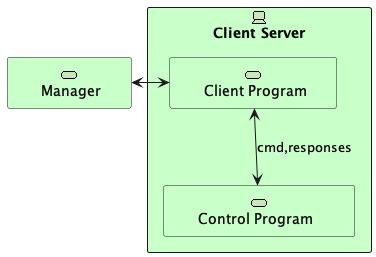
\includegraphics[height=0.2\textheight]{./part/Proyecto_ejecutivo/memoria_descriptiva/descripcionDelProyecto/client/uml/clientServerConcept}
    \caption{Diagrama UML de despliegue del cliente}\label{fig:Diagrama UML de despliegue del cliente}
\end{figure}

\subparagraph{Dominio}

Este programa está compuesto principalmente de infraestructura.
Esto es debido a que una vez recibido el comando mediante el RPC sólo será necesario ejecutarlo.
Siendo tarea del programa ejecutado interpretar dicho comando y transformar esa cadena de caracteres que contiene el \textit{Step} a un dominio interno.
Por ejemplo, el programa cliente contenido en un sistema UNIX de LINUX podrá ejecutar cualquier comando de consola contenido por defecto:

\begin{verbatim}
    ./runMyComand --arg=arg1 --argN=argN
\end{verbatim}

Este ejemplo será la cadena de caracteres contenida en el \textit{Step} guardado en el Manager y recibido por el \textit{Client} que ejecutará en el mismo sistema operativo.
Las posibilidades son tantas como comandos haya instalados en el servidor cliente.
En el sistema será posible mandar a ejecutar todos los comandos que acepte el programa de control para interactuar con el motor de corriente continua.
Algunos de los posibles comandos serán:

\begin{verbatim}
    ./pidControl --velocity=30rpm
    ./pidControl --position=180deg
    ./pidControl --setP=1
    ./pidControl --setI=0
    ./pidControl --setD=0
    ./pidControl --enabled=true
    ./pidControl --enabled=false
\end{verbatim}

El diagrama de Dominio de el \textit{Client} de la \cref{fig:Diagrama UML de el dominio de cliente} muestra dos Value Objects para los \textit{Steps} recibidos y para los \textit{Results} obtenidos.
No hay \textit{Entities} al no necesitar persistencia.

\begin{figure}[H]
    \centering
    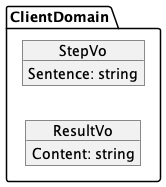
\includegraphics[height=0.2\textheight]{./part/Proyecto_ejecutivo/memoria_descriptiva/descripcionDelProyecto/client/uml/clientDomain}
    \caption{Diagrama UML de el dominio de cliente}\label{fig:Diagrama UML de el dominio de cliente}
\end{figure}

\subparagraph{Casos de uso}

\begin{itemize}
    \item \textbf{Execute Unary Step}: La descripción de este caso de uso se centra en un ejemplo de nuestro programa de control.
    Servirá, por ejemplo, para establecer una consigna de control para el PID\@.
    En la~\cref{fig:Use Case-Execute Unary Step} se aprecia el diagrama de flujo correspondiente.

    \begin{verbatim}
    ./pidControl --velocity=30rpm
    \end{verbatim}

    \begin{figure}[H]
        \centering
        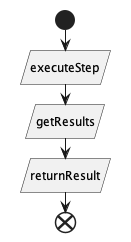
\includegraphics[height=0.25\textheight]{./part/Proyecto_ejecutivo/memoria_descriptiva/descripcionDelProyecto/client/uml/executeUnaryStep}
        \caption{Use Case: Execute Unary Step}\label{fig:Use Case-Execute Unary Step}
    \end{figure}

    \item \textbf{Execute ClientStream Step}

    Será de utilidad, por ejemplo, para establecer una configuración completa con una sola llamada para nuestro PID\@.
    En la~\cref{fig:Use Case-Execute ClientStream Step} se aprecia el diagrama de flujo correspondiente.
    \begin{verbatim}
    ./pidControl --velocity=30rpm
    ./pidControl --position=180deg
    ./pidControl --setP=1
    ./pidControl --setI=0
    ./pidControl --setD=0
    \end{verbatim}

    \begin{figure}[H]
        \centering
        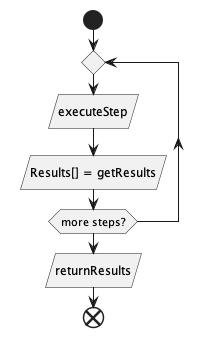
\includegraphics[height=0.25\textheight]{./part/Proyecto_ejecutivo/memoria_descriptiva/descripcionDelProyecto/client/uml/executeClientStreamStep}
        \caption{Use Case: Execute ClientStream Step}\label{fig:Use Case-Execute ClientStream Step}
    \end{figure}

    \item \textbf{Execute ServerStream Step}

    Será utilizado para habilitar el control pid durante un determinado tiempo e ir devolviendo el estado la variable controlada en tiempo real.

    \begin{verbatim}
    ./pidControl --enabled=true --time=10s
    \end{verbatim}

    O dejar el control activado indefinidamente hasta que llegue otra request de tipo Unary que lo detenga

    \begin{verbatim}
    ./pidControl --enabled=false
    \end{verbatim}

    En la~\cref{fig:Use Case-Execute ServerStream Step} se muestra el diagrama de flujo.

    \begin{figure}[H]
        \centering
        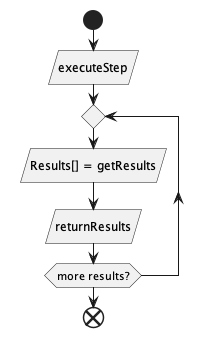
\includegraphics[height=0.25\textheight]{./part/Proyecto_ejecutivo/memoria_descriptiva/descripcionDelProyecto/client/uml/executeServerStreamStep}
        \caption{Use Case: Execute ServerStream Step}\label{fig:Use Case-Execute ServerStream Step}
    \end{figure}

    \item \textbf{Execute Bidirectional Step}

    \begin{figure}[H]
        \centering
        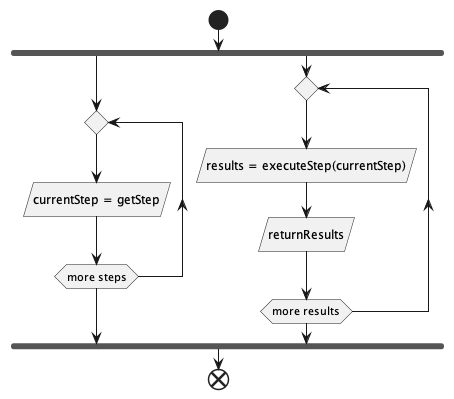
\includegraphics[height=0.25\textheight]{./part/Proyecto_ejecutivo/memoria_descriptiva/descripcionDelProyecto/client/uml/executeBidiStep}
        \caption{Use Case: Execute Bidirectional Step}\label{fig:Use Case-Execute Bidirectional Step}
    \end{figure}
\end{itemize}

\subparagraph{Estructura de carpetas}
    En el proyecto constará de 4 carpetas principales

\tiny
\dirtree{%
    .1 Project .
        .2 Domain.
        .2 Application.
        .2 Adapter.
        .2 Bootstrap.
}
\normalsize

\textbf{Dominio}

\begin{figure}[H]
    \tiny
\dirtree{%
    .1 Domain.
        .2 Step.
            .3 StepVo.
            .3 Repository.
                .4 consoleWrite.
            .3 Services.
                .4 Executor.
        .2 Result.
            .3 ResultVo.
}
\normalsize
    \caption[Diagrama de objetos de dominio]{}\label{fig:1-ClientDomainFolderStructure}
\end{figure}

\textbf{Aplicación}

\tiny
\dirtree{%
.1 Application.
    .2 Port.
        .3 in.
            .4 Step.
                .5 Execute.
                    .6 Command.
                    .6 UseCase.
}
\normalsize

\textbf{Adapters}

\tiny
\dirtree{%
    .1 Adapter.
        .2 in.
            .3 GRPC.
                .4 Harán uso de los useCases de aplicación cuando llegue una request RPC.
            .3 Console.
                .4 Por ejemplo si quisieramos ejecutar los casos de uso mediante terminal.
        .2 out.
            .3 console.
                .4 implementación de los repository de llamada a los servidores clientes.
}
\normalsize





